\documentclass{article}
\usepackage[utf8]{inputenc}
\usepackage[margin=0.35in]{geometry}


\title{Cyber Security Pracitcal 3}
\author{Shane Cincotta }
\date{May 5 2020}

\usepackage{natbib}
\usepackage{graphicx}

\begin{document}

\maketitle

% \begin{figure}[h!]
% \centering
% 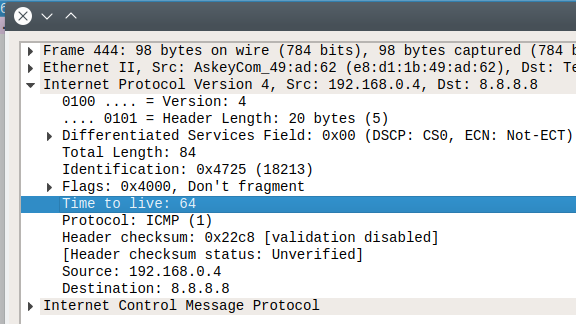
\includegraphics[scale=0.65]{Q1.png}
% \caption{}
% \end{figure}

\section*{Q1}
\begin{figure}[h!]
\centering
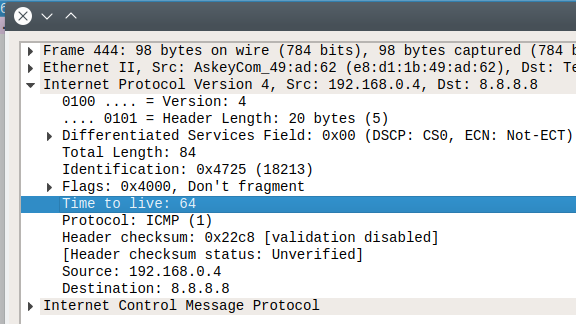
\includegraphics[scale=0.5]{Q1.png}
\caption{}
\end{figure}

\section*{Q2}
\begin{figure}[h!]
\centering
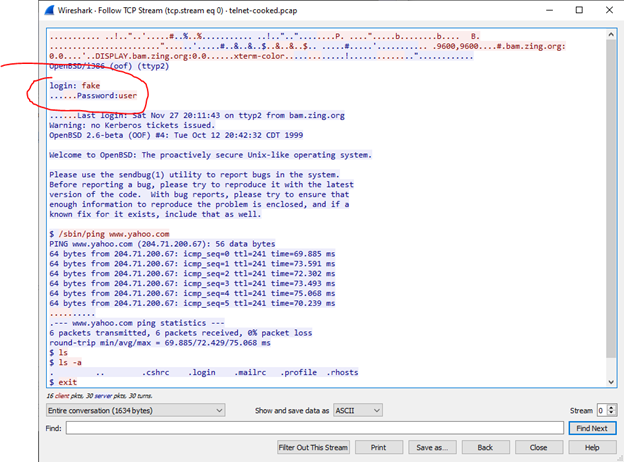
\includegraphics[scale=0.5]{Q2.png}
\caption{}
\end{figure}
\clearpage

\section*{Q3}
According to figure 3, ciper suite TLS\_ECDHE\_RSA\_WITH\_AES\_128\_GCM\_SHA256 is used.\\
\begin{figure}[h!]
\centering
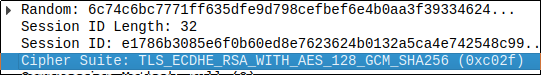
\includegraphics[scale=0.5]{Q3.png}
\caption{}
\end{figure}

\section*{Q4}
\begin{figure}[h!]
\centering
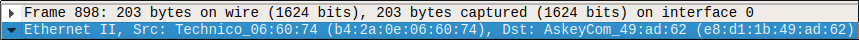
\includegraphics[scale=0.5]{Q4a.png}
\caption{}
\end{figure}

\begin{figure}[h!]
\centering
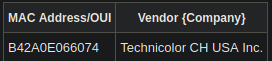
\includegraphics[scale=0.5]{Q4b.png}
\caption{}
\end{figure}

\begin{figure}[h!]
\centering
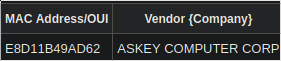
\includegraphics[scale=0.5]{Q4c.png}
\caption{}
\end{figure}

\section*{Q5}
According to figure 7, the message that is being exchanged is "who has 192.168.0.3? Tell 192.168.0.1", other than this, the ARP message "192.168.1.1 is at 48:a4:72:b052:07" is also exchanged.\\
\begin{figure}[h!]
\centering

\includegraphics[scale=0.5]{Q5a.png}
\caption{}
\end{figure}
\clearpage

\section*{Q6}
\begin{figure}[h!]
\centering
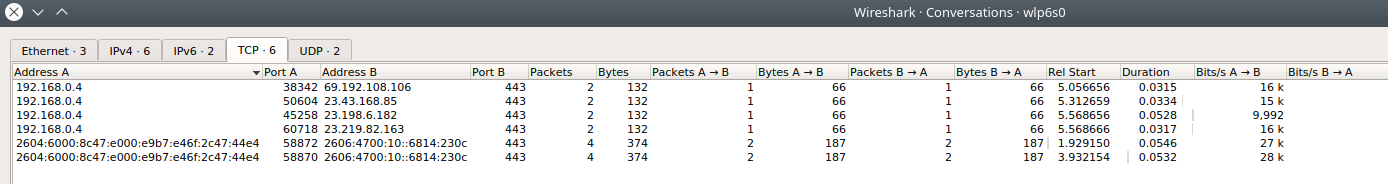
\includegraphics[scale=0.4]{Q6a.png}
\caption{}
\end{figure}

\begin{figure}[h!]
\centering
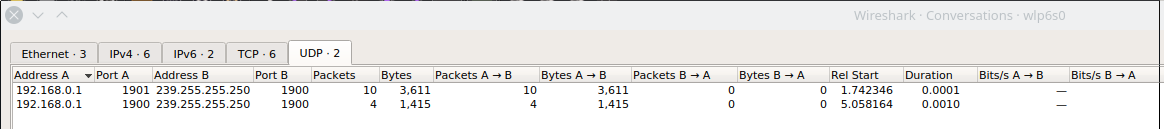
\includegraphics[scale=0.4]{Q6b.png}
\caption{}
\end{figure}
\clearpage

\section*{Q7}
\begin{figure}[h!]
\centering
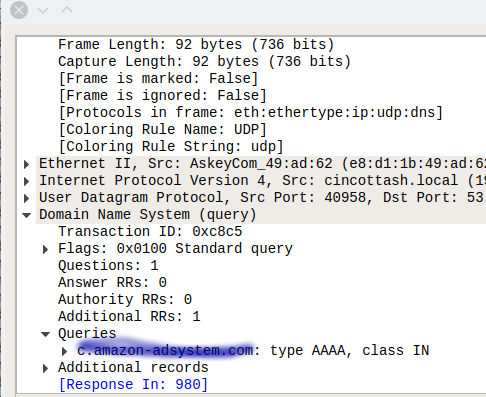
\includegraphics[scale=0.4]{Q7a.png}
\caption{}
\end{figure}

\begin{figure}[h!]
\centering
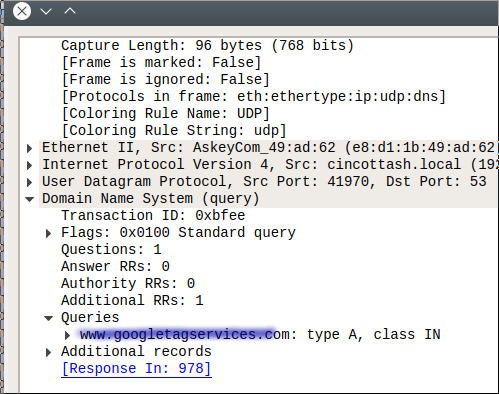
\includegraphics[scale=0.4]{Q7b.png}
\caption{}
\end{figure}

\begin{figure}[h!]
\centering
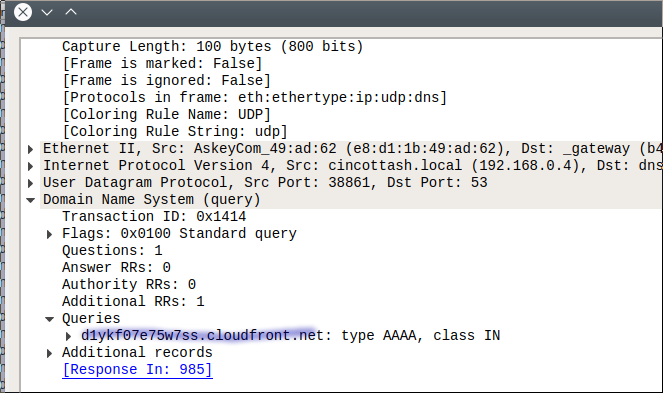
\includegraphics[scale=0.4]{Q7c.png}
\caption{}
\end{figure}
\clearpage

\section*{Q8}
IP address provided to VM1 by the DHCP server, and the IP address mask (or prefix length) provided to VM1 by the DHCP server.\\
\begin{figure}[h!]
\centering

\includegraphics[scale=1.0]{Q8a.png}
\caption{}
\end{figure}

\begin{figure}[h!]
\centering

\includegraphics[scale=1.0]{Q8b.png}
\caption{}
\end{figure}

DNS address provided to VM1 by the DHCP server, and the default route (e.g. router) address provided to VM1 by the DHCP server.\\
\begin{figure}[h!]
\centering
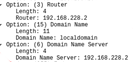
\includegraphics[scale=1.0]{Q8c.png}
\caption{}
\end{figure}

\end{document}